%%%%%%%%%%%%%%%%%%%%%%%%%%%%%%%%%%%%%%%%%
% University Assignment Title Page
% LaTeX Template
% Version 1.0 (27/12/12)
%
% This template has been downloaded from:
% http://www.LaTeXTemplates.com
%
% Original author:
% WikiBooks (http://en.wikibooks.org/wiki/LaTeX/Title_Creation)
%
% License:
% CC BY-NC-SA 3.0 (http://creativecommons.org/licenses/by-nc-sa/3.0/)
%
% Instructions for using this template:
% This title page is capable of being compiled as is. This is not useful for
% including it in another document. To do this, you have two options:
%
% 1) Copy/paste everything between \begin{document} and \end{document}
% starting at \begin{titlepage} and paste this into another LaTeX file where you
% want your title page.
% OR
% 2) Remove everything outside the \begin{titlepage} and \end{titlepage} and
% move this file to the same directory as the LaTeX file you wish to add it to.
% Then add \input{./title_page_1.tex} to your LaTeX file where you want your
% title page.
%
%%%%%%%%%%%%%%%%%%%%%%%%%%%%%%%%%%%%%%%%%
%\title{Title page with logo}
%----------------------------------------------------------------------------------------
%	PACKAGES AND OTHER DOCUMENT CONFIGURATIONS
%----------------------------------------------------------------------------------------

\documentclass[12pt]{article}
\usepackage[toc,page]{appendix}
\usepackage[spanish]{babel}
\usepackage[utf8x]{inputenc}
\usepackage{amsmath}
\usepackage{graphicx}
\usepackage{fancyhdr}
\usepackage[colorinlistoftodos]{todonotes}
\usepackage{changepage}
\usepackage[font=scriptsize]{caption}
\usepackage[a4paper,bindingoffset=0.2in,left=1in,right=1in,top=1in,bottom=0.5in,footskip=.25in]{geometry}
\usepackage{cleveref}
\usepackage[hidelinks]{hyperref}
\usepackage{eurosym}
\usepackage{MathUnicode}
\usepackage{amsmath}
\usepackage{amssymb}
\usepackage{amsthm}
\usepackage{pdfsync}
\usepackage{color,xspace,hyperref}
\usepackage{changepage}
\usepackage{float}
\usepackage{caption}



\setlength{\arrayrulewidth}{1mm}
\setlength{\tabcolsep}{18pt}
\renewcommand{\arraystretch}{1.5}


\renewcommand{\labelitemii}{$\circ$}
\pagestyle{fancy}
\lhead{\textbf{Teoría del caos y fractales}}
\chead{\leftmark}
%\rhead{\includegraphics[width=2.8cm]{img/logo_memo}}
\rhead{\textbf{CyC}}

\newtheorem{theorem}{Teorema}
\newtheorem{lemma}{Lema}
\newtheorem{proposition}{Proposición}
\theoremstyle{definition}
\newtheorem{definition}{Definición}
\newtheorem{example}{Ejemplo}

\renewcommand{\headrulewidth}{0.5pt}

\begin{document}

\begin{titlepage}

\newcommand{\HRule}{\rule{\linewidth}{0.5mm}} % Defines a new command for the horizontal lines, change thickness here

\center % Center everything on the page

%----------------------------------------------------------------------------------------
%	HEADING SECTIONS
%----------------------------------------------------------------------------------------

\textsc{\LARGE Universidad Autónoma de Madrid}\\[1.5cm] % Name of your university/college
\textsc{\Large Complejidad y Computación}\\[0.5cm] % Major heading such as course name


%----------------------------------------------------------------------------------------
%	TITLE SECTION
%----------------------------------------------------------------------------------------

\HRule \\[0.4cm]
{ \huge \bfseries Teoría del Caos y fractales}\\[0.4cm] % Title of your document
\HRule \\[1cm]


%----------------------------------------------------------------------------------------
%	AUTHOR SECTION
%----------------------------------------------------------------------------------------


% If you don't want a supervisor, uncomment the two lines below and remove the section above
\Large \emph{Autoress:}\\
Alejandro \textsc{Villegas}\\ % Your name
Elena \textsc{Gutiérrez}\\ % Your name
Miguel Ángle \textsc{González-gallego} \\
Pedro \textsc{Valero}\\[1cm] % Your name

%----------------------------------------------------------------------------------------
%	LOGO SECTION
%----------------------------------------------------------------------------------------

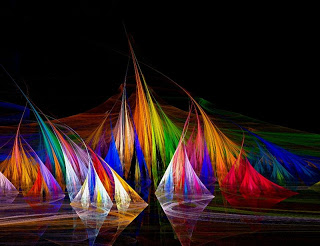
\includegraphics{img/Logo.jpg}\\ % Include a department/university logo - this will require the graphicx package

%----------------------------------------------------------------------------------------
%	DATE SECTION
%----------------------------------------------------------------------------------------

{\large \today}\\[1cm] % Date, change the \today to a set date if you want to be precise


%----------------------------------------------------------------------------------------

\vfill % Fill the rest of the page with whitespace

\end{titlepage}

\tableofcontents
\newpage

\section{Introducción}
Antes de comenzar a indagar en los fundamentos de la Teoría del Caos o en los fractales, debemos aclarar una serie de conceptos que aparecerán a lo largo de estos apuntes.

\begin{definition}[Teoría del Caos]
La teoría del Caos es la rama de las Matemáticas que estudia el comportamiento de sistemas dinámicos \textbf{deterministas} muy sensibles a los datos iniciales.
\end{definition}

Es importante destacar el hecho de que los sistemas han de ser deterministas pues, de lo contrario, estaríamos hablando de procesos aleatorios o impredecibles. La \textbf{idea clave} del concepto del Caos es que comprendemos el fenómeno y sabemos modelizarlo ``a la perfección'' pero el resultado futuro varía enormemente a partir de un pequeño cambio en los valores tomados del mundo real.

\begin{example}
A modo de ejemplo podemos suponer un fenomeno que venga modelizado por la ecuación:
\[z_{n+1} = f(z_n) \text{ siendo } f(x) = x^2+1\]

Para un $n=11$, que no parece ser algo demasiado grande, siendo $z$ un número complejo, supongamos que cometemos un error muy pequeño, de la forma: $ε=10^{-5}+10^{-5}i$ al medir $z_0$.

En estas condiciones, la diferencia entre el valor obtenido y el original es
\[f^{11}(ε)=1.4 \cdot 10^{181} + 1.13\cdot 10^{174}\]
\end{example}

También es fundamental aclarar, aunque algunos lectores pueden tener ya una idea intuitiva, qué es un fractal.

\begin{definition}[Fractal]
Un fractal es un objeto geométrico cuya estructura básica, fragmentada o irregular, se repite a diferentes escalas.
\end{definition}

\section{Sistemas discretos}
Tiempo estimado de esta parte: 50 min\\
Referencia
\begin{itemize}
\item The Beauty of fractals temas 1,2,3,4 y 8.
\end{itemize}
\subsection{Ecuaciones en diferencias.}
\subsection{Procesos de Verhulst. Period doubling, bifurcaciones.}
\subsection{Ecuación logística}
\subsection{$x=x^2+c$. Julia sets. Mandelbrot set.}
\subsection{Fractales/dimensión de Hausdorlf/dimensión fractal}
\subsection{Polvo de Cantor} No aparece en The Beauty of fractals (en algún otro libro de la bibliografía está).
\subsection{Ecuaciones de Volterra}

%%%%%%%%%%%%%%%%%%%%%%%%%%%%%%%%%%%%%%%%%%%%%%%%%%%%%%%%%%
%%%%%%%%%%%%%%%%%%%%%%%%%%%%%%%%%%%%%%%%%%%%%%%%%%%%%%%%%%
%%%%%%%%%%%%%%%%%%%%%%%%%%%%%%%%%%%%%%%%%%%%%%%%%%%%%%%%%%
%%%%%%%%%%%%%%%%%%%%%%%%%%%%%%%%%%%%%%%%%%%%%%%%%%%%%%%%%%
%%%%%%%%%%%%%%%%%%%%%%%%%%%%%%%%%%%%%%%%%%%%%%%%%%%%%%%%%%
%%%%%%%%%%%%%%%%%%%%%%%%%%%%%%%%%%%%%%%%%%%%%%%%%%%%%%%%%%
%%%%%%%%%%%%%%%%%%%%%%%%%%%%%%%%%%%%%%%%%%%%%%%%%%%%%%%%%%
%%%%%%%%%%%%%%%%%%%%%%%%%%%%%%%%%%%%%%%%%%%%%%%%%%%%%%%%%%
%%%%%%%%%%%%%%%%%%%%%%%%%%%%%%%%%%%%%%%%%%%%%%%%%%%%%%%%%%

\section{Sistemas continuos}
% Tiempo estimado de esta parte: 70 min.\\
% Referencia
% \begin{itemize}
% \item CHAOS: An introduction to dynamical systems temas 7,8,9 y 11.
% \item Elegant Chaos
% \end{itemize}

\subsection{Sistemas dinámicos deterministas, ecuaciones diferenciales}
\subsection{Espacio de estados/fases}
\subsection{Oscilaciones}
\subsection{Sistemas disipativos: atractores}
\subsection{Flujos, compresibles o no}
\subsection{Atractores extraños: caos}
Hay que hablar de Atractores de Lorentz (artículo relacionado)
\subsection{Exponentes de lyapunov}
Hay que incluir algo.
\subsection{Ejemplos de sistemas}
Para los ejemplos: Non linear dynamic and chaos.
\subsection{Lorenz Volterra}
Ecuaciones en Non linear dynamic and chaos.

%%%%%%%%%%%%%%%%%%%%%%%%%%%%%%%%%%%%%%%%%%%%%%%%%%%%%%%%%%
%%%%%%%%%%%%%%%%%%%%%%%%%%%%%%%%%%%%%%%%%%%%%%%%%%%%%%%%%%
%%%%%%%%%%%%%%%%%%%%%%%%%%%%%%%%%%%%%%%%%%%%%%%%%%%%%%%%%%
%%%%%%%%%%%%%%%%%%%%%%%%%%%%%%%%%%%%%%%%%%%%%%%%%%%%%%%%%%
%%%%%%%%%%%%%%%%%%%%%%%%%%%%%%%%%%%%%%%%%%%%%%%%%%%%%%%%%%
%%%%%%%%%%%%%%%%%%%%%%%%%%%%%%%%%%%%%%%%%%%%%%%%%%%%%%%%%%
%%%%%%%%%%%%%%%%%%%%%%%%%%%%%%%%%%%%%%%%%%%%%%%%%%%%%%%%%%
%%%%%%%%%%%%%%%%%%%%%%%%%%%%%%%%%%%%%%%%%%%%%%%%%%%%%%%%%%
%%%%%%%%%%%%%%%%%%%%%%%%%%%%%%%%%%%%%%%%%%%%%%%%%%%%%%%%%%

\section{Aplicaciones}
Tiempo estimado de esta parte: 30 min.\\
Referencia
\begin{itemize}
\item Guide to Chaos
\end{itemize}
\subsection{Generación gráfica de conjuntos de Julia}
\subsection{Ejemplos gráficos de explorar el conjunto de Mandelbrot}
\subsection{Caos y criptografía}
\subsection{Compresión fractal}
\subsection{Antenas fractales}
\subsection{Aeronáutica y fluidos}

%%%%%%%%%%%%%%%%%%%%%%%%%%%%%
%%%%%%
%%%%%%
%%%%%%
%%%%%%%%%%%%%%%%%%%%%%%%%%%%%
\newpage

\begin{thebibliography}{1}
\bibitem{B1165 SPR}Dprott, J.C, Elegant Chaos
\bibitem{C4260 PEI}Peitgen, H-O, Richter, P.H., The Beauty of Fractals.
\bibitem{B1165 NEW}Hall, Nina, Guide to Chaos
\bibitem{B0240 STR}Strogatz, S.H. Nonlinear Dynamics and Chaos,
\bibitem{B1165 ALL}Alligood, K.T. et al, CHAOS: An introduction to dynamical systems
\end{thebibliography}

\end{document}